\documentclass{article}
\usepackage{amsmath}
\usepackage{amsfonts}
\usepackage{bm}
\usepackage{graphicx}
\usepackage{float}
\usepackage{subfigure}
\usepackage{enumitem}
\usepackage{ctex}

\renewcommand{\figurename}{Figure}
\renewcommand{\thesubfigure}{}

\begin{document}
\begin{titlepage}
\vspace*{\fill}
\begin{center}
\huge Wireless Communication Systems \\HW4\\ 109064509 楊暐之
\end{center}
\vspace{\fill}
\end{titlepage}

\begin{flushleft}
For simplicity, I use the same random data of channel to simulate the bit error probability for each cases.\\
Due to coherent detection, the phase is irrelevant for SC,MRC and EGC. We only care about the energy gain of these three cases.
Otherwise, to determine the bit error probability of QPSK, we only need to know the received SNR.\\
For the first and second parts, I show the simulated results, and all discussion are left for the third part \\[0.5cm]
\begin{enumerate}
% Rayleigh fading
	{\Large \item  \bf Rayleigh fading}\\
	I generate the energe gain of  Rayleigh fading by directly using raylrnd according to the given SNR,and generate uniform random phase 
	\begin{enumerate}
		\item  Selective Combining\\
			\begin{figure}[H]
			\centering
			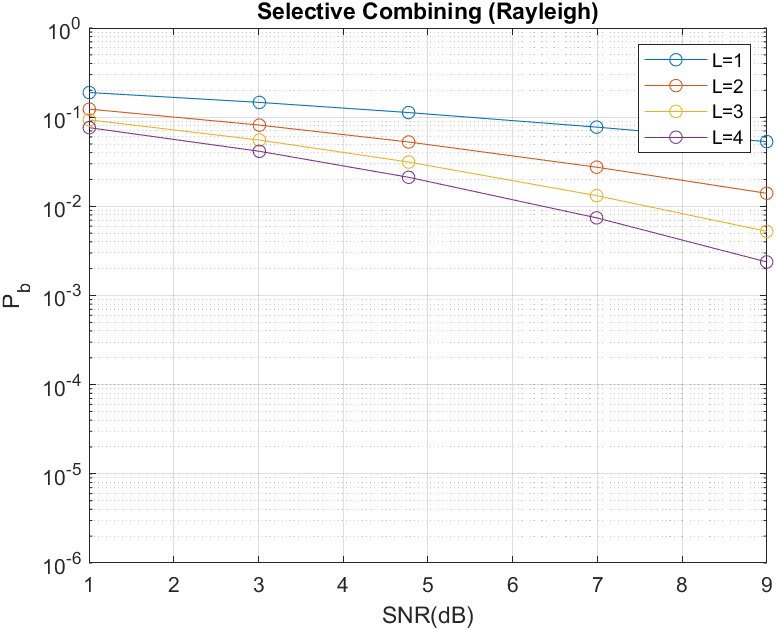
\includegraphics[width=0.9\textwidth, height=0.44\textheight]{Rayleigh_SC}
			\end{figure}
\newpage
		\item Maximal Ratio Combining\\
			\begin{figure}[H]
			\centering
			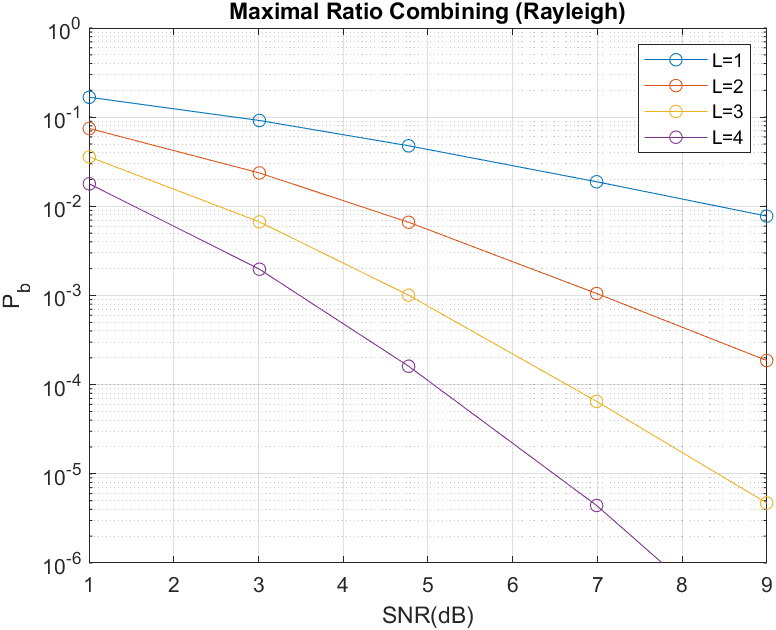
\includegraphics[width=0.9\textwidth, height=0.4\textheight]{Rayleigh_MRC}
			\end{figure}
		\item Equal Gain Combining\\
			\begin{figure}[H]
			\centering
			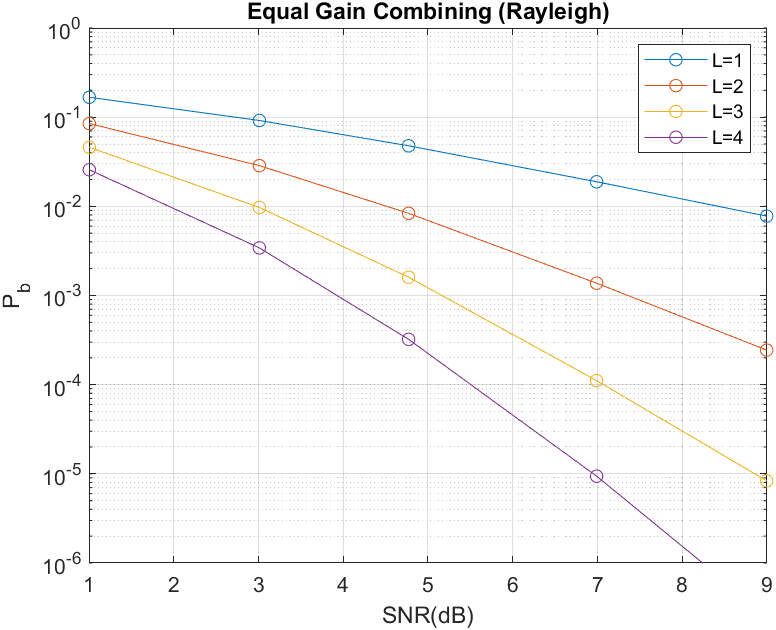
\includegraphics[width=0.9\textwidth, height=0.4\textheight]{Rayleigh_EGC}
			\end{figure}
\newpage
		\item Direct Combining\\
			\begin{figure}[H]
			\centering
			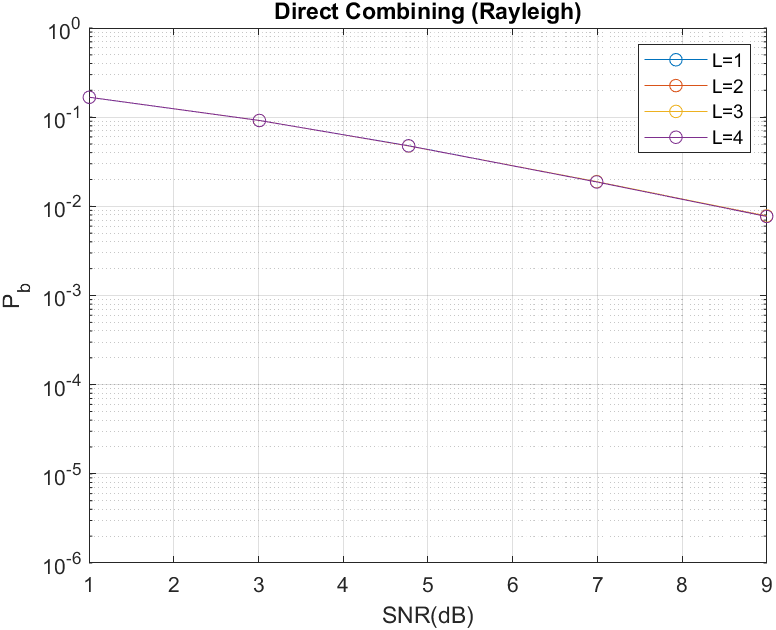
\includegraphics[width=0.9\textwidth, height=0.4\textheight]{Rayleigh_DC}
			\end{figure}
	\end{enumerate}
\newpage
% Rician fading
	{\Large \item  \bf Rician fading}\\
	I use two Gaussian random variable to generate the Rician fading gain according to given SNR
	\begin{enumerate}
		\item  Selective Combining\\
			\begin{figure}[H]
			\centering
			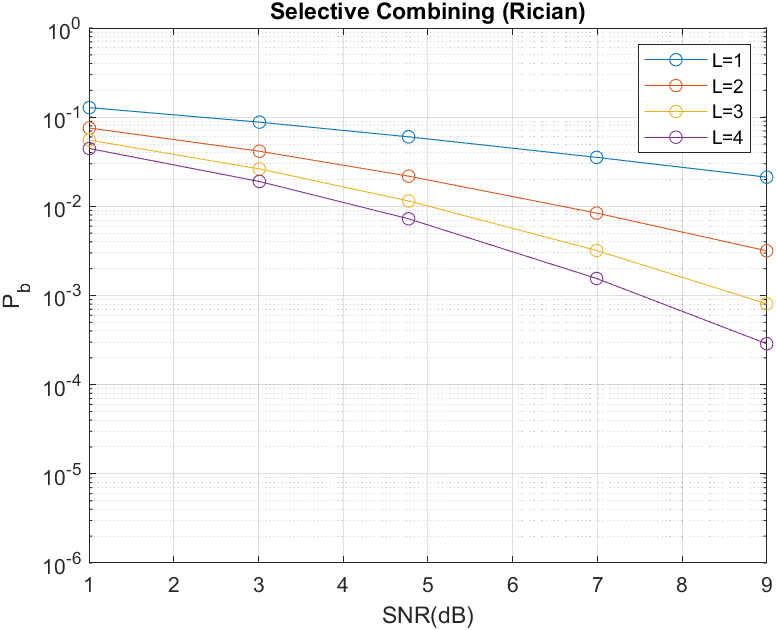
\includegraphics[width=0.9\textwidth, height=0.4\textheight]{Rician_SC}
			\end{figure}
\newpage
		\item Maximal Ratio Combining\\
			\begin{figure}[H]
			\centering
			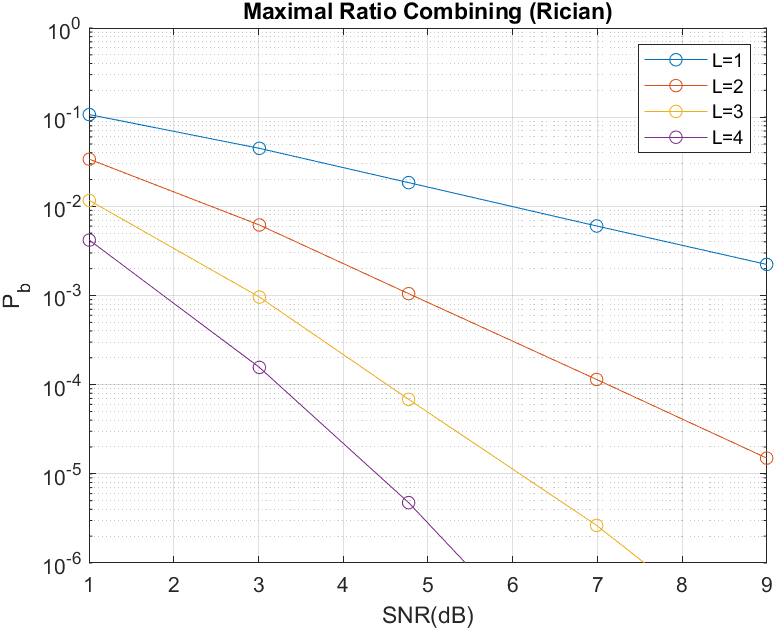
\includegraphics[width=0.9\textwidth, height=0.4\textheight]{Rician_MRC}
			\end{figure}
		\item Equal Gain Combining\\
			\begin{figure}[H]
			\centering
			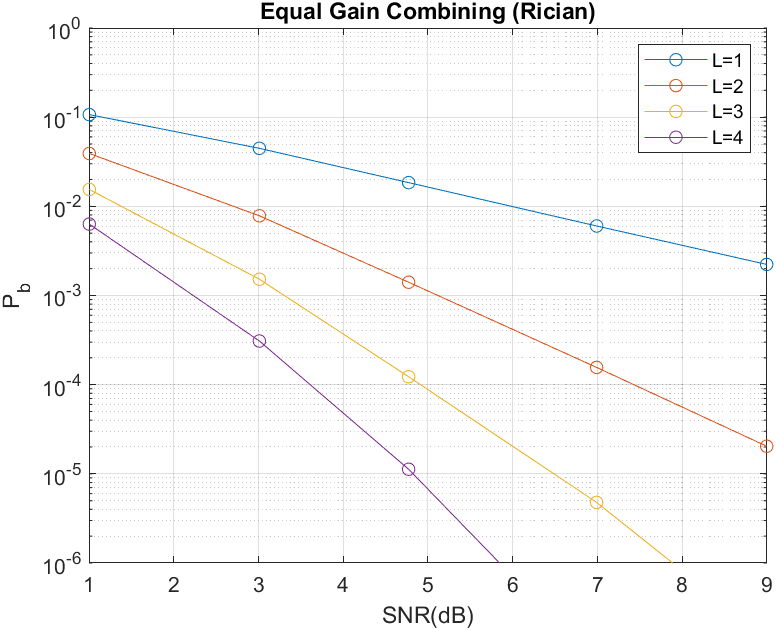
\includegraphics[width=0.9\textwidth, height=0.4\textheight]{Rician_EGC}
			\end{figure}
\newpage
		\item Direct Combining\\
			\begin{figure}[H]
			\centering
			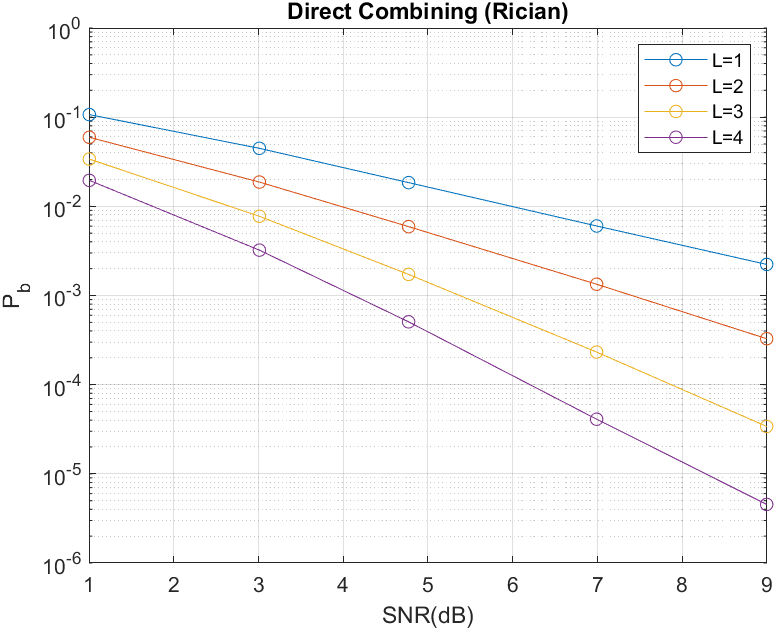
\includegraphics[width=0.9\textwidth, height=0.4\textheight]{Rician_DC}
			\end{figure}
	\end{enumerate}
	{\Large \item  \bf Comparison and discussion }\\
	For SC, since we only choose the path that receives max SNR, the improvement of BER is not significant.\\
	For MRC and EGC, these two cases are performed much better than SC, but they pay more cost in complexity.\\
	For DC of  Rayleigh fading channel, since the phase of Rayleigh fading channel is uniform in $[0,2\pi]$, the value of $\cos\theta$ and  $\sin\theta$ are 	concentrated at $\pm1$. Thus, directly combine received signals of $L$ paths almost do not improve the performance. And this situation does not 			occur for Rician fading channel.\\
	By the way, since the Los component exist for Ricean fading, the performance of Ricean fading is better than Rayleigh fading for each cases.
\end{enumerate}
\end{flushleft}



\end{document}